\documentclass{beamer}
\usetheme{metropolis} 
\title{\huge Konobi}
\date{}
\subtitle{Software Development Methods project}
\author{Lorenzo Basile, Irene Brugnara, Roberto Corti, Arianna Tasciotti}
\usepackage{caption}
\begin{document}
  \maketitle
  \section{Introduction}
  \begin{frame}{Our project}
    The goal of our project was to develop a command line version of \textbf{Konobi}, a board game for two players. The project also contains a client-server version of the game.
    \vspace{0.7cm}
    \pause
    \\What tools did we use?
    \begin{itemize}
    \item Java 15
    \item Gradle
    \item TravisCI
    \item Git \& GitHub
    \end{itemize}
    \end{frame}
  \begin{frame}{Konobi}
    Konobi is a drawless game and it can be played either on a go board or a chess board.
    \\Two players, black and white, take turns at placing stones of their color on the board, starting with black. The aim of the players is to build chains of connected stones of their color.
    \vspace{0.5cm}
    \pause
    \\The game is won by the first player who connects the two opposite edges of the board.
    \begin{itemize}
    \item Black: top $\leftrightarrow$ bottom
    \item White: left $\leftrightarrow$ right
    \end{itemize}
      \end{frame}
      
     \begin{frame}{Connections}
     Two like-colored stones are:
     \vspace{0.5cm}
    \begin{columns}
			\column{0.5\textwidth}
			\begin{figure}
				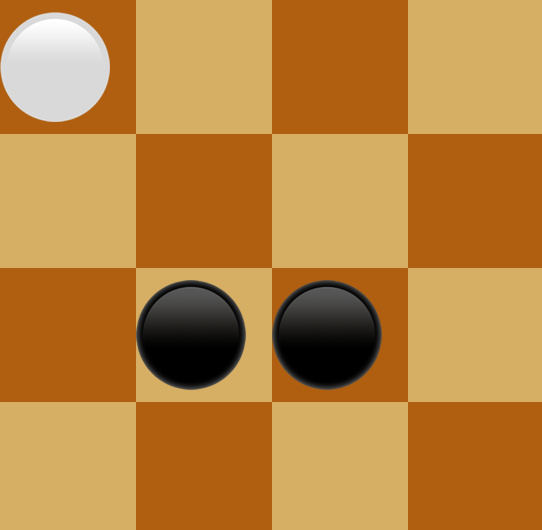
\includegraphics[scale=0.35]{images/strong.png}
				\caption*{Strongly connected}
			\end{figure}
					
			\column{0.5\textwidth}
			\begin{figure}
				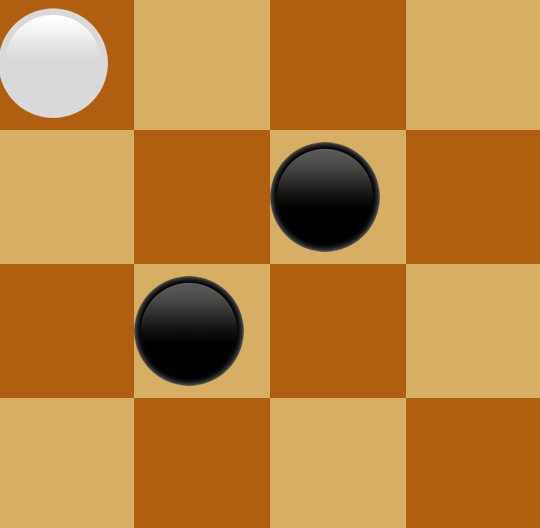
\includegraphics[scale=0.35]{images/weak.png}
				\caption*{Weakly connected}
			\end{figure}
		
	\end{columns}
	\vspace{0.7cm}
	A chain is a set of connected stones

      \end{frame}
      
      \begin{frame}{Placement rules}
     Not all moves are allowed:
     \begin{itemize}
     \item \textbf{Weak connections} to a certain stone are illegal unless it is impossible to make a placement that is both strongly connected to that stone and not weakly connected to another
     \item \textbf{Crosscut} placements are always illegal
     \end{itemize}
    \begin{columns}
			\column{0.5\textwidth}
			\begin{figure}
				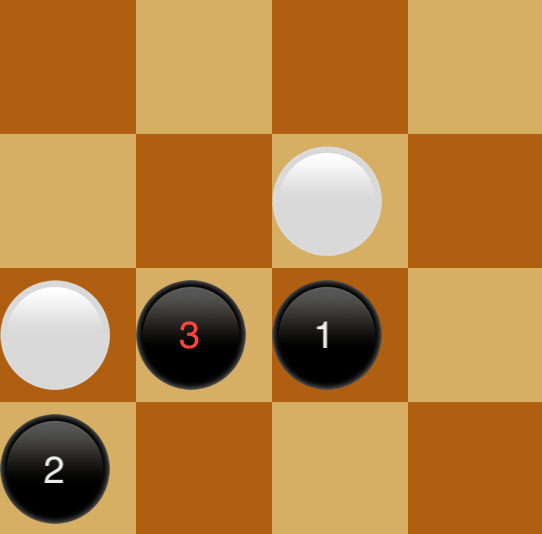
\includegraphics[scale=0.35]{images/legal_weak.png}
				\caption*{Legal weak connection}
			\end{figure}
					
			\column{0.5\textwidth}
			\begin{figure}
				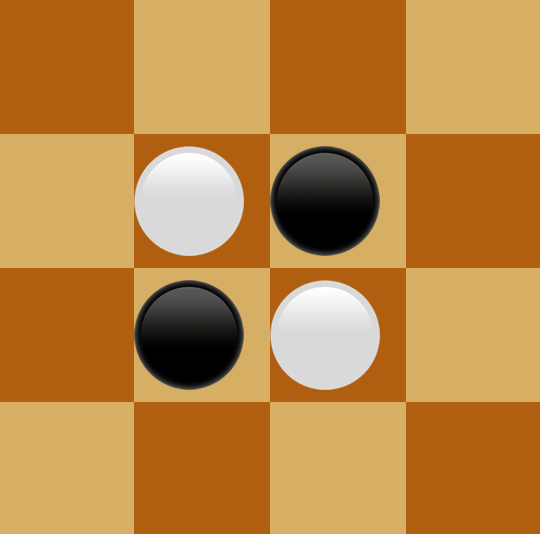
\includegraphics[scale=0.35]{images/crosscut.png}
				\caption*{Crosscut placement}
			\end{figure}
		
	\end{columns}
      \end{frame}
      
      \begin{frame}{Additional rules}
     \begin{itemize}
     \item \textbf{Pie rule}: at his first move, white can decide to switch colors with black instead of making a move
     \item \textbf{Mandatory pass}: if a player cannot make a move (because of placement restrictions), he has to pass
     \end{itemize}
      \end{frame}
     
\end{document}